\documentclass[10pt,letterpaper]{article}
\usepackage{amsmath,amssymb,geometry,graphicx}
\usepackage{enumitem}
%\settextfont{B Nazanin}
\usepackage{lipsum}
\setlength{\parskip}{3mm}
\setlength{\parindent}{0mm}
\newcommand{\wid}{0.49\textwidth}
\newcommand{\widone}{60mm}
\begin{document}
\Large
\begin{center}
In the name of beauty

11th problem set solution of ComNet course

\hrulefill
\end{center}
Q1) 
\begin{enumerate}[label=\alph*-]
\item
SSL is technically built in application layer (that is why an application program, willing to use SSL, would load sufficient libraries), but it is thought of as a transport layer protocol from a developer point of view, due to providing sockets just like TCP (and UDP of course).
\item
Sequence numbering is a technique to prevent an intruder from re-ordering segments by preserving packet orders, which should albeit, be encrypted through hash functions to keep them private from the intruder (such that the intruder cannot manipulate it).
\item
IPsec (network-layer security) is conceived to provide “blanket coverage” because of its capability of encrypting datagrams payload, regardless of what they exactly are, which leads to keeping all the underlying content hidden from any third-party.
\item
The SPD indicates what types of datagrams (as a function of source IP
address, destination IP address, and protocol type) are to be IPsec processed; and
for those that are to be IPsec processed, which security association should be used. In a sense, the
information in a SPD indicates “what” to do with an arriving datagram.
\end{enumerate}

Q2) 
\begin{enumerate}[label=\alph*-]
\item
When a duplicate key is used, in a chosen-plaintext attack taken by Trudy against Alice, Trudy can request a message from Alice, which is encrypted by a key. Trudy is able to get to the key by XOR operations, thus compromising plain texts from any cipher-texts later sent by Alice and encrypted by \textit{this} duplicate key. 
\item
The MK is a shared secret known
only to the client and the authentication server, which they each use to generate
a second key, the Pairwise Master Key (PMK). The authentication server then
sends the PMK to the AP. Hence, the client and AP
now have a shared key and have mutually authenticated each other.
\item
Such a weak security scheme would also ban the legitimate TCP connections. A solution is performing blocking by distinguishing suspicious source IP addresses or port numbers.
\end{enumerate}

Q3) 

\begin{enumerate}[label=\alph*-]

\item
\begin{figure}[htbp]
\centering
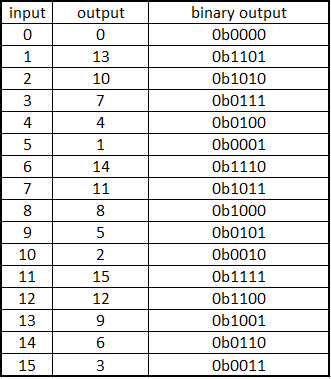
\includegraphics[width=70mm]{Table_10.png}
\end{figure}
As seen, the outputs are unique.
\item
\begin{figure}[htbp]
\centering
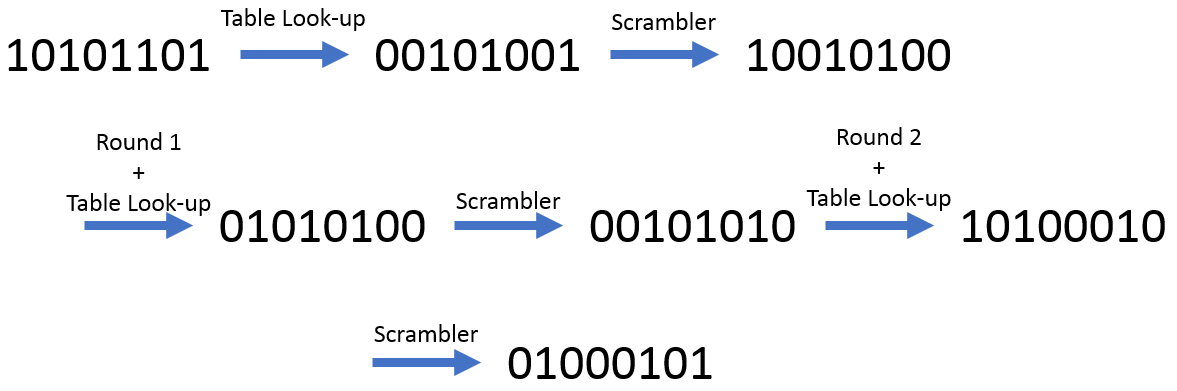
\includegraphics[width=100mm]{Trans.png}
\end{figure}
\item
Any number, say $z$, coprime to 16 can be replaced instead of 13 since
$$
x\equiv y\mod 16\iff zx\equiv zy\mod 16
$$
\end{enumerate}



Q4) The intruder, having the hash output at hand, can find the number of digits equal to $0,1,2,\cdots ,9$, but does not know their arrangement. The best he can do, is to arrange a digit of each of 1, 2, 4, 5 and 6 and three digits of 3 randomly. He ends up with a total of 
$
{8!\over 1!\times1!\times3!\times1!\times1!\times1!}=6720
$
 different cases and his probability of detection becomes ${1\over 6720}\approx 1.5\times 10^{-4}$.


Q5) 

The little Fermat's theorem implies
%\begin{theorem}
$$
a^p\equiv a\mod p\quad,\quad p\text{ is prime}
$$
which reduces to
$$
a^{p-1}\equiv 1\mod p\quad,\quad p\text{ is prime}
$$
when $\gcd(a,p)=1$. Also, we use another theorem to conclude the final answer, implying that if $a\equiv b\mod p$ and $a\equiv b\mod q$ when $p$ and $q$ are primes, then
%\begin{theorem}
$$
a\equiv b\mod pq
$$
%\end{theorem}
Alice's encryption:
\begin{equation}\begin{split}
c=m^e\mod n=2^{13}\mod 77=8192\mod 77=30
\end{split}\end{equation}
Bob's decryption:
\begin{equation}\begin{split}
\hat m=c^d\mod 77=30^{37}\mod 77
\end{split}\end{equation}
We know that
\begin{equation}\begin{split}
&30^6\equiv 1\mod 7
\\&
30^{10}\equiv 1\mod 11
\end{split}\end{equation}
therefore
\begin{equation}\begin{split}
&30^{36}\equiv 1\mod 7
\\&
30^{30}\equiv 1\mod 11
\end{split}\end{equation}
and
\begin{equation}\begin{split}
&30^{37}\equiv 30\equiv2\mod 7
\\&
30^{37}\equiv 30^7\equiv (-3)^7
\\&
\equiv -3\times 27^2
\\&
\equiv -3\times 5^2
\\&
\equiv -75
\\&
\equiv 2\mod 11
\end{split}\end{equation}
since
\begin{equation}\begin{split}
&30^{37}\equiv 2\mod 7
\\&30^{37}\equiv 2\mod 11
\end{split}\end{equation}
we conclude that
$$
30^{37}\equiv 2\mod 77
$$
and therefore, Bob can decrypt Alice's message uniquely.

Jake's decryption:
\begin{equation}\begin{split}
\hat m=c^d\mod 77=30^{97}\mod 77
\end{split}\end{equation}
We know that
\begin{equation}\begin{split}
&30^{6}\equiv 1\mod 7
\\&
30^{10}\equiv 1\mod 11
\end{split}\end{equation}
therefore
\begin{equation}\begin{split}
&30^{96}\equiv 1\mod 7
\\&
30^{90}\equiv 1\mod 11
\end{split}\end{equation}
and
\begin{equation}\begin{split}
&30^{37}\equiv 30\equiv2\mod 7
\\&
30^{97}\equiv 30^7\equiv (-3)^7
\\&
\equiv -3\times 27^2
\\&
\equiv -3\times 5^2
\\&
\equiv -75
\\&
\equiv 2\mod 11
\end{split}\end{equation}
since
\begin{equation}\begin{split}
&30^{97}\equiv 2\mod 7
\\&30^{97}\equiv 2\mod 11
\end{split}\end{equation}
we conclude that
$$
30^{97}\equiv 2\mod 77
$$
and therefore, Jake can decrypt Alice's message uniquely.
\newline\newline
b. To show (4)$\implies$(3), assume by contrary that $\gcd(e,z)\ne 1$. Then, $x\in \Bbb Z$ and $x>1$ exists such that $\gcd(e,z)=x$ which means that $x|e$ and $x|z$. Since condition (4) holds, we have
\begin{equation}\begin{split}
z|ed-1&\implies x|ed-1
\\&
\implies x|xq-1\quad,\quad\text{for some }q\in\Bbb Z
\\&
\implies x|-1
\end{split}\end{equation}
which is a contradiction. Hence (3) must hold in order for (4) to hold and the proof is complete $\blacksquare$

Q6)

\begin{enumerate}[label=\alph*-]
\item
\begin{figure}[htbp]
\centering
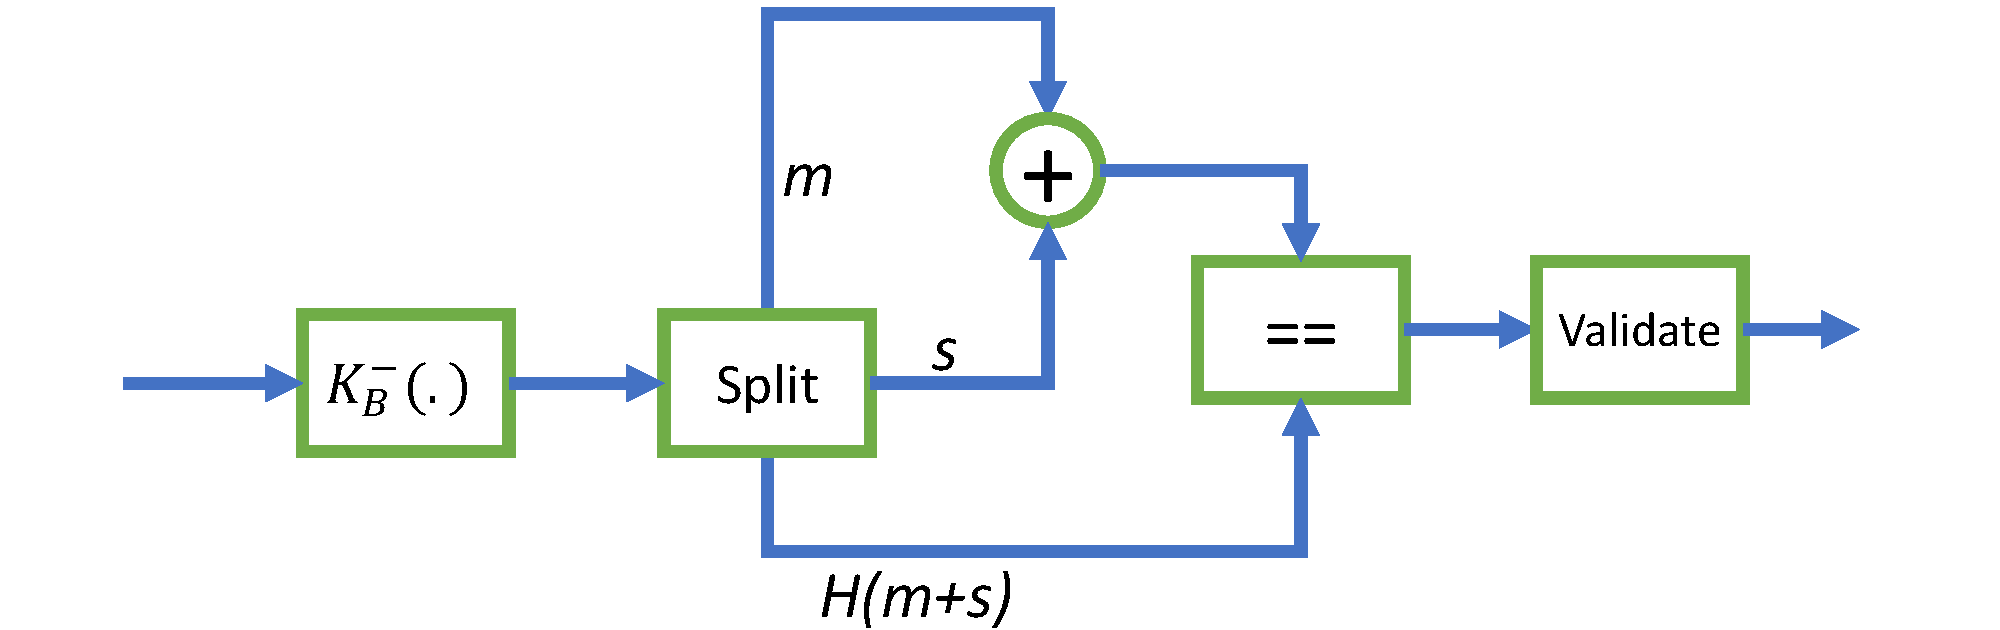
\includegraphics[width=140mm]{decrypt.pdf}
\end{figure}
\item
Neither end-to-end authentication nor message integrity have been preserved since an intruder can emulate all the process and initiate a fake message.

\item
\begin{figure}[htbp]
\centering
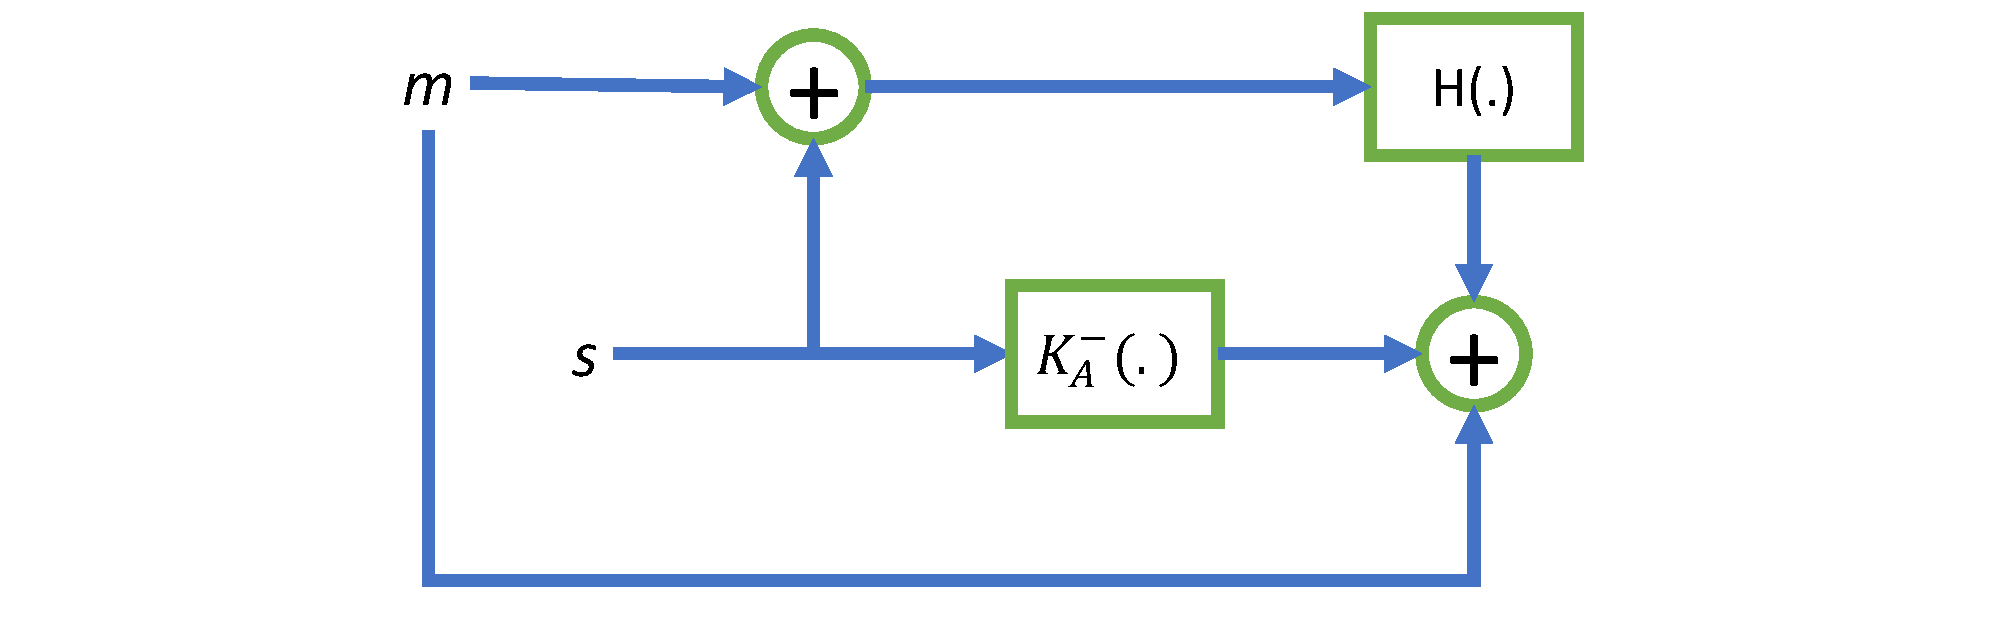
\includegraphics[width=140mm]{enc_mod.pdf}
\end{figure}
\end{enumerate}
\end{document}